\documentclass[tikz,border=10pt]{standalone}
\begin{document}
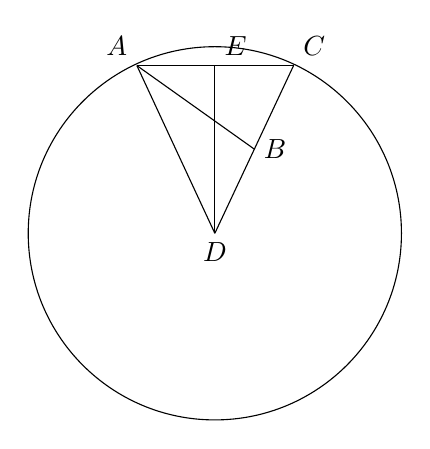
\begin{tikzpicture}
  \coordinate (D) at (0,0);
  \coordinate (A) at (-0.99,2.13);
  \coordinate (C) at (1.00,2.13);
  \coordinate (B) at (0.50,1.07);
  \coordinate (E) at (0,2.13);

  \draw (D) circle (2.37);

  \draw (A) -- (C);
  \draw (A) -- (B);
  \draw (A) -- (D);
  \draw (C) -- (D);
  \draw (D) -- (E);

  \node[above left] at (A) {$A$};
  \node[above right] at (C) {$C$};
  \node[right] at (B) {$B$};
  \node[above right] at (E) {$E$};
  \node[below] at (D) {$D$};
\end{tikzpicture}
\end{document}
